\documentclass[preview]{standalone}

\usepackage{amsmath}
\usepackage{amssymb}
\usepackage{tikz}
\usepackage{stellar}
\usepackage{definitions}
\usepackage{bettelini}

\begin{document}

\id{geofisica-rotazione-terra}
\genpage

\section{Rotazione della terra}

\plain{Vi sono più velocità di rotazioni: i punti su diversi cerchi di latitudine hanno diverse velocità di rotazione rispetto al centro della terra.}

\begin{snippetdefinition}{forza-di-coriolis}{Forza di Coriolis}
    A causa del moto di rotazione attorno al proprio asse,
    gli oggetti che non sono ancorati alle terra si spostano verso destra rispetto alla loro direzione di spostamento.
    La forza di Coriolis si applica solo alla componente dello spostamento che è perpendicolare all'equatore.
\end{snippetdefinition}

\plain{La forza di Coriolis è alla base della formazione dei sistemi ciclonici o anticiclonici nell'atmosfera.}

\begin{snippet}{forza-coriolis-illustration}
    \begin{center}
        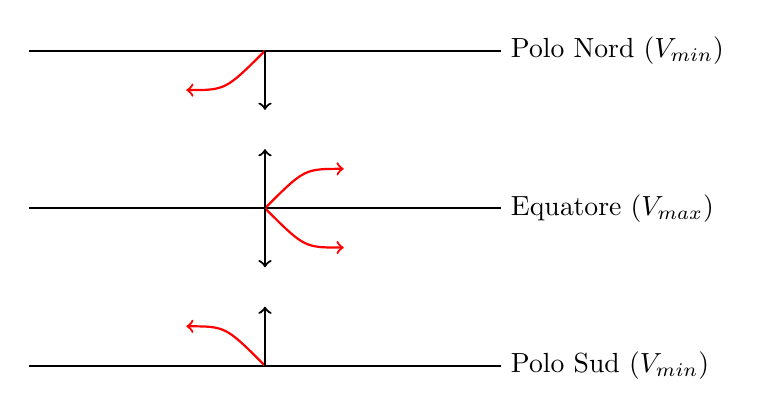
\begin{tikzpicture}
            % Diagramma Polo Nord
            \draw[thick] (0,2) -- (6,2);
            \draw[->, red, thick] (3,2) .. controls (2.5,1.5) .. (2,1.5);
            \draw[->, black, thick] (3,2) -- (3,1.25);
            \node[right] at (6,2) {Polo Nord ($V_{min}$)};
            
            % Diagramma Equatore
            \draw[thick] (0,0) -- (6,0);
            \draw[->, red, thick] (3,0) .. controls (3.5,-0.5) .. (4,-0.5);
            \draw[->, black, thick] (3,0) -- (3,-0.75);
            \draw[->, red, thick] (3,0) .. controls (3.5,0.5) .. (4,0.5);
            \draw[->, black, thick] (3,0) -- (3,0.75);
            \node[right] at (6,0) {Equatore ($V_{max}$)};
            
            % Diagramma Polo Sud
            \draw[thick] (0,-2) -- (6,-2);
            \draw[->, red, thick] (3,-2) .. controls (2.5,-1.5) .. (2,-1.5);
            \draw[->, black, thick] (3,-2) -- (3,-1.25);
            \node[right] at (6,-2) {Polo Sud ($V_{min}$)};
        \end{tikzpicture}
    \end{center}
\end{snippet}

\end{document}